\section{Hardware}
\label{Sec:5-hardware}
%\subsection{XBeee: configuração}

\subsection{Raspberry - Sistema Operacional}

Raspberry Pi é um computador, como tal é possível usá-lo sobre um sistema operacional. O sistema operacional usado é o Raspian, baseado no Debian customizado para rodar no raspberry pi. Apesar de teoricamente não ser necessário o raspberry usar um sistema operacional, facilita muito o desenvolvimento tal equipamento conter uma interface amigável para seu uso.

\subsection{Raspberry - Adaptador Wifi}

Após o sistema Raspian ser instalado no cartão de memória, foi necessário configurar o adaptador Wifi. O modelo usado é o TP-Link TL-WN723N.

%\subsubsection{Procedimentos}
%\begin{lstlisting}
%wget https://dl.dropboxusercontent.com/u/80256631/8188eu-3.18.11-v7-781.tar.gz
%tar xzf 8188eu-3.18.11-v7-781.tar.gz
%./install.sh
%\end{lstlisting}

\begin{figure}[H]
\centering
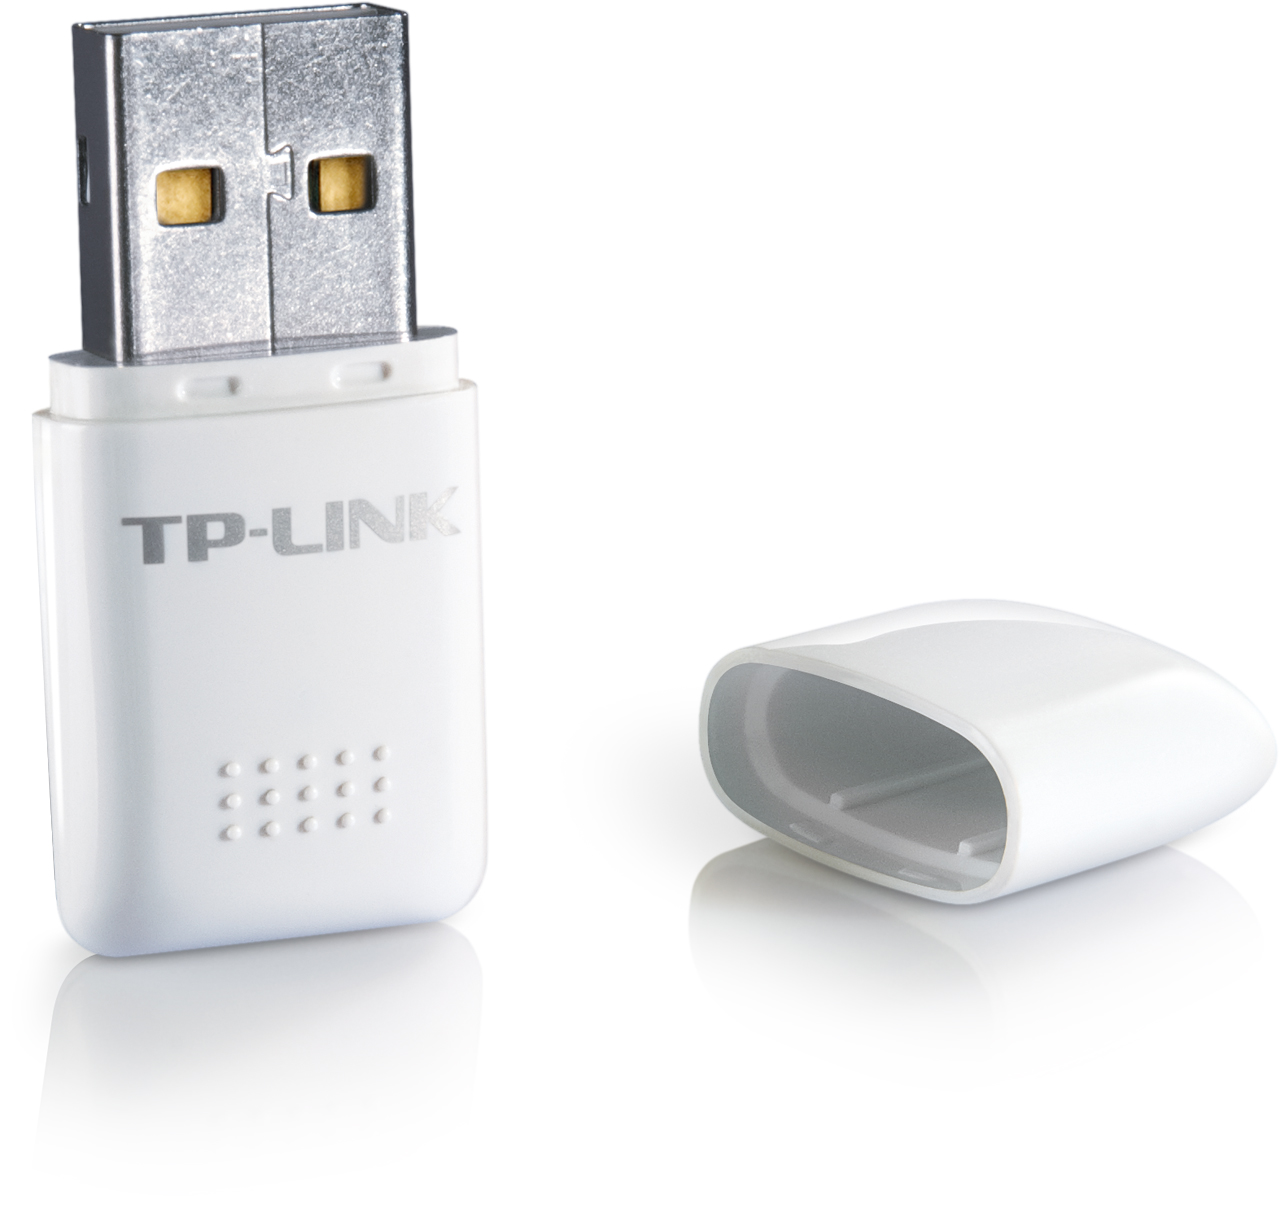
\includegraphics[width=5cm,height=5cm,keepaspectratio]{figuras/wifi-adapter.jpg}
\caption{\label{fig:wifi-adapter} Adaptador wifi usado no raspberry}
\end{figure}

\subsection{Raspberry x Arduino: comunicação}

Para testar a comunicação entre o Módulo Coordenador (figura \ref{fig:teste-inicial-raspberry}) e o módulo sensor (figura \ref{fig:teste-inicial-arduino}), foi montado o esquema representado na figura \ref{fig:teste-inicial-all} e foram executados dois programas. O programa \ref{lst:teste-inicial-arduino} foi utilizado no módulo sensor para transmitir o valor "123123" por um datagrama a ser enviado pela rede do XBee. Já o programa \ref{lst:teste-inicial-raspberry} foi utilizado no Módulo Coordenador para receber o datagrama ZigBee e imprimir no console do Raspberry.

\begin{figure}[H]
\centering
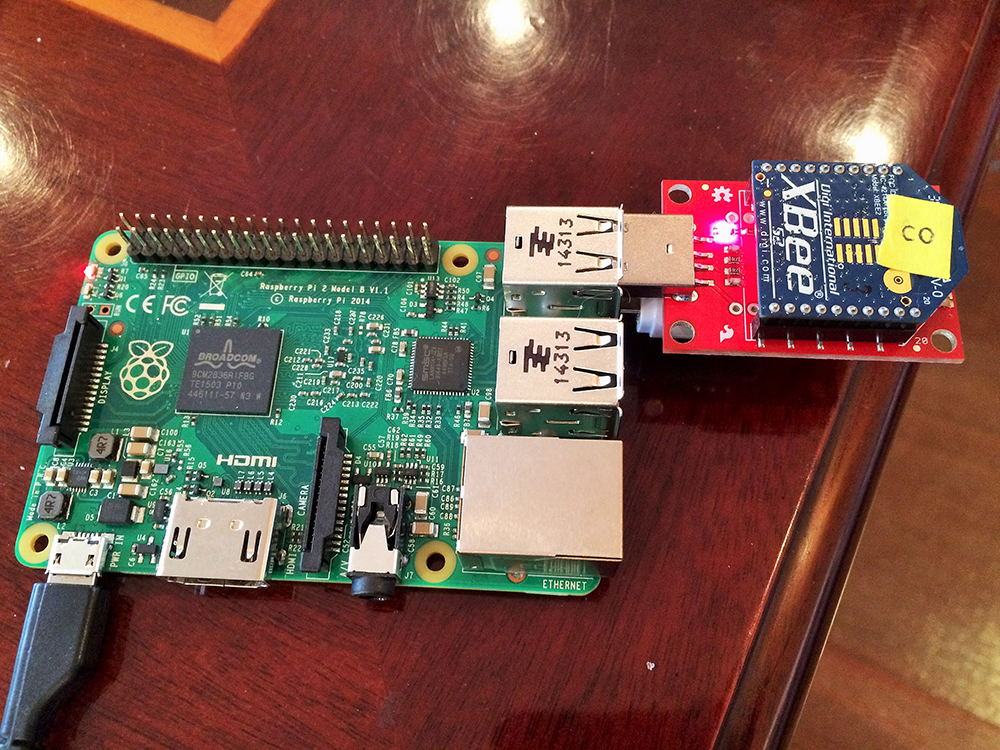
\includegraphics[width=7cm,keepaspectratio]{figuras/teste-inicial-raspberry.jpg}
\caption{\label{fig:teste-inicial-raspberry} Teste de comunicação: Módulo Coordenador}
\end{figure}

\begin{figure}[H]
\centering
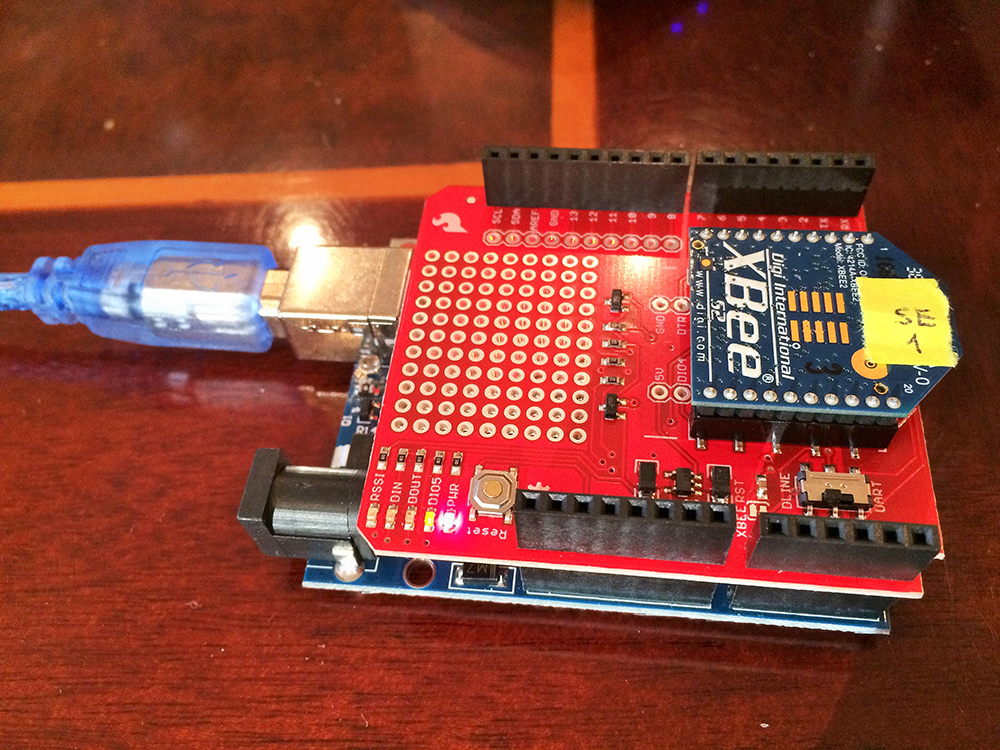
\includegraphics[width=7cm,keepaspectratio]{figuras/teste-inicial-arduino.jpg} 
\caption{\label{fig:teste-inicial-arduino} Teste de comunicação: Módulo Sensor}
\end{figure}

\begin{figure}[H]
\centering
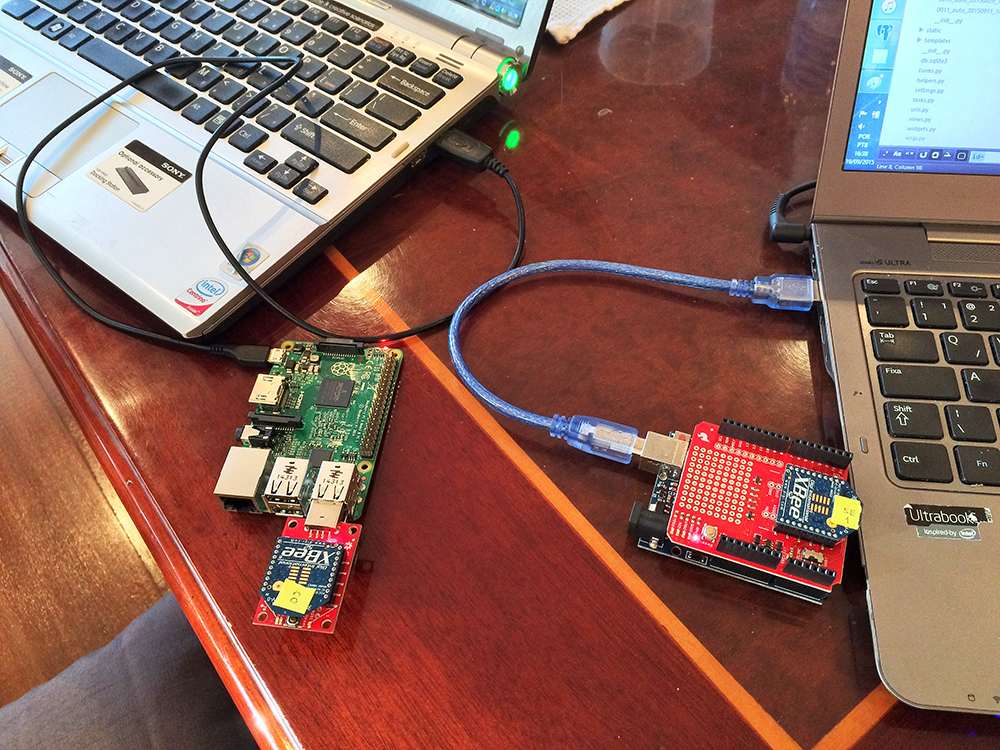
\includegraphics[width=7cm,keepaspectratio]{figuras/teste-inicial-all.jpg} 
\caption{\label{fig:teste-inicial-all} Teste de comunicação: Montagem}
\end{figure}

\lstinputlisting[language=C, caption=teste-inicial-arduino.c, label={lst:teste-inicial-arduino}]{Anexos/teste-inicial-arduino.c}

\lstinputlisting[language=Python, caption=teste-inicial-raspberry.py, label={lst:teste-inicial-raspberry}]{Anexos/teste-inicial-raspberry.py}

\begin{figure}[H]
\centering
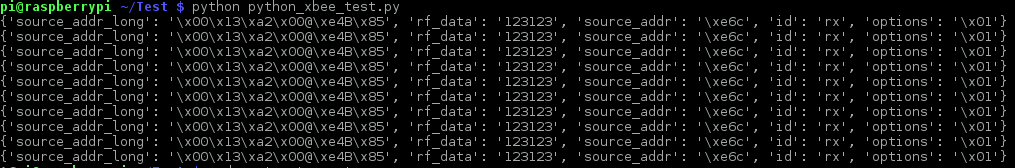
\includegraphics[width=1\textwidth]{figuras/teste-inicial-raspberry-arduino.png}
\caption{\label{fig:raspberry-arduino-1} Teste de comunicação Raspberry e Arduino}
\end{figure}

Uma rota foi criada no sistema na parte web para receber requisições de cadastro de consumo pelo módulo coordenador. O objetivo do segundo teste foi detectar a presença do sensor na rede e cadastrá-lo caso não estivessem registrado no banco de dados. Além disso foi necessário verificar que existe um equipamento associado àquele sensor, caso contrário, o sistema não aceitará o registrao de consumos.
Para isso, o programa do primeiro teste foi reescrito para receber o pacote e então enviá-lo via http para cadastrar o consumo teste.

\begin{figure}[H]
\centering
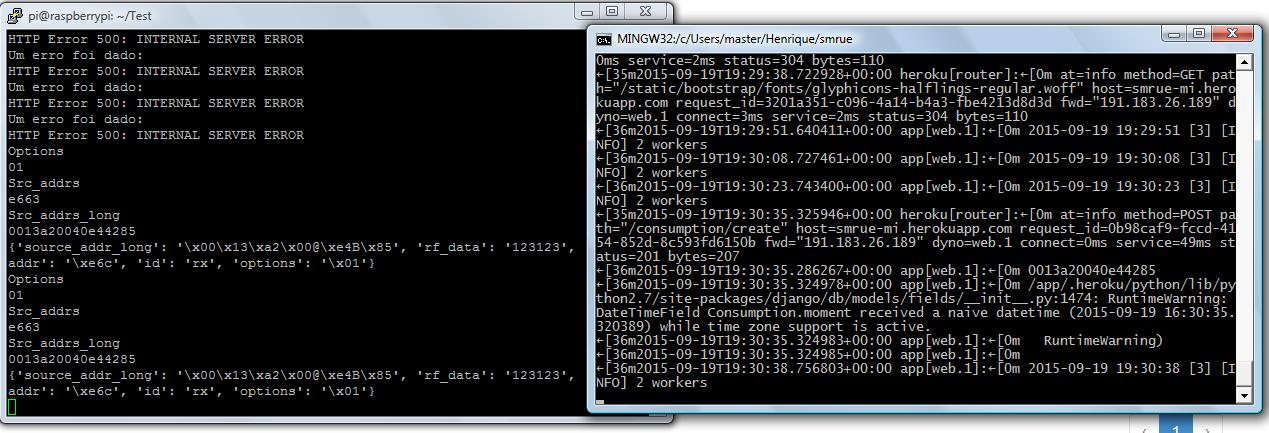
\includegraphics[width=1\textwidth]{figuras/sensor_creation.jpg}
\caption{\label{fig:sensor_creation} Teste de criação de sensor e de consumo }
\end{figure}

Em um primeiro momento, quando o sensor nem está no sistema,  o servidor retorna um erro HTTP 500 (erro de servidor), isso porque apesar do sensor ter sido criado no sistema, este não está vinculado a nenhum equipamento. Após vincular o sensor a um equipamento na tela de configurações, pode-se ver que o servidor então retorna um status 201, que mostra que o consumo foi criado.


